%Préambule du document :
\documentclass[12pt]{report}
\usepackage[top=2cm,bottom=2cm,left=2cm,right=2cm]{geometry}
\usepackage[utf8]{inputenc}
\usepackage[francais]{babel}
\usepackage{color}
\usepackage{graphicx} 
\usepackage{url}
\usepackage{hyperref}
\usepackage[T1]{fontenc}
\usepackage{float}

\usepackage{listingsutf8} % ne change rien, a virer ?

% pour code source
\usepackage{listings}
\lstset{
	basicstyle=\footnotesize,
	%extendedchars=\true
	%inputencoding=utf8/latin1
	numberstyle=\footnotesize,
	frame=single,
	tabsize=2,
	breaklines=true,
	numbers=left,
	rulecolor=,
	keywordstyle=\color[rgb]{0,0,1},
	commentstyle=\color[rgb]{0.133,0.545,0.133},
	stringstyle=\color[rgb]{0.627,0.126,0.941},
}

\definecolor{red1}{RGB}{153,0,0}

\hypersetup{colorlinks,%
            citecolor=black,%
            filecolor=black,%
            linkcolor=black,%
            urlcolor=red1}


%Page de Garde
\makeatletter
\def\clap#1{\hbox to 0pt{\hss #1\hss}}%
\def\ligne#1{%
\hbox to \hsize{%
\vbox{\centering #1}}}%
\def\haut#1#2#3{%
\hbox to \hsize{%
\rlap{\vtop{\raggedright #1}}%
\hss
\clap{\vtop{\centering #2}}%
\hss
\llap{\vtop{\raggedleft #3}}}}%
\def\bas#1#2#3{%
\hbox to \hsize{%
\rlap{\vbox{\raggedright #1}}%
\hss
\clap{\vbox{\centering #2}}%
\hss
\llap{\vbox{\raggedleft #3}}}}%
\def\maketitle{%
\thispagestyle{empty}\vbox to \vsize{%
\haut{}{\@blurb}{}
\vfill
\vspace{1cm}
\begin{flushleft}
\usefont{OT1}{ptm}{m}{n}
\huge \@title
\end{flushleft}
\par
\hrule height 4pt
\par
\begin{flushright}
\usefont{OT1}{phv}{m}{n}
\Large \@author
\par
\end{flushright}
\vspace{1cm}
\vfill
\vfill
\bas{}{\@location, le \@date}{}
}%
\cleardoublepage
}
\def\date#1{\def\@date{#1}}
\def\author#1{\def\@author{#1}}
\def\title#1{\def\@title{#1}}
\def\location#1{\def\@location{#1}}
\def\blurb#1{\def\@blurb{#1}}
\date{\today}
\author{}
\title{}
\location{Nancy}\blurb{}
\makeatother
\title{\textcolor[RGB]{153,0,0}{Systèmes de fichiers distribué : comparaison de GlusterFS, MooseFS et Ceph avec déploiement sur la grille de calcul Grid’5000.}}
\author{Jean-François Garçia, Florent Lévigne,\\Maxime Douheret, Vincent Claudel.}
\location{Nancy}
\blurb{%
IUT Nancy-Charlemagne Université Nancy 2\\
\textbf{\textcolor[RGB]{153,0,0}{Licence Pro Asrall}}\\[1em]
Tuteur : Maître de Conférences : Lucas Nussbaum\\
}% 


%definition des pages
\makeatletter
\def\thickhrulefill{\leavevmode \leaders
\hrule height 1ex \hfill \kern \z@}
\def\@makechapterhead#1{%
\vspace*{10\p@}%
{\parindent \z@
{\reset@font
\usefont{OT1}{phv}{m}{n}
\LARGE Partie \thechapter\par\nobreak}%
\par\nobreak
\vspace*{30\p@}
\interlinepenalty\@M
\usefont{OT1}{ptm}{b}{n}
{\raggedright \Huge \bfseries #1}%
\par\nobreak
\vskip 20\p@
\hrule height 2pt
\par\nobreak
\vskip 45\p@
}}
\def\@makeschapterhead#1{%
\vspace*{10\p@}%
{\parindent \z@
{\raggedleft \reset@font
\scshape \vphantom{\@chapapp{} \thechapter}
\par\nobreak}%
\par\nobreak
\vspace*{30\p@}
\interlinepenalty\@M
\usefont{OT1}{ptm}{b}{n}
{\raggedright \Huge \bfseries #1}%
\par\nobreak
\par\nobreak
\vskip 45\p@
}} 



%Corps du document :
\begin{document}
	\maketitle
	\tableofcontents

	\chapter{Introduction}
		\section{Contexte}
			Étudiants en licence professionnelle ASRALL (Administration de Systèmes, Réseaux, et Applications à base de Logiciels libres),
			notre formation prévoie une période de x mois à mis temps pour la réalisation d'un projet tuteuré.

			Le projet que nous avons choisis consiste à comparer diverses solutions de systèmes de fichiers distribué.

		\section{Système de fichiers distribué}
			% Très fortement inspiré de Wikipédia (citer sources en fin de rapport)
			% système de fichier distribué basé sur un fs "normal" ?
			Un système de fichiers (file system en anglais) est une façon de stocker des informations et de les organiser dans des fichiers,
			sur des périphérique comme un disque dur, un CD-ROM, une clé USB, etc.
			Il existe de nombreux systèmes de fichiers (certains ayant des avantages sur d'autres),
			dont entre autre l'ext (Extented FS), le NTFS (New Technology FileSystem), ZFS (Zettabyte FS), FAT (File Allocation Table).
			
			Un système de fichiers distribué est un système de fichiers permettant le partage de données à plusieurs clients
			au travers du réseau.
			Contrairement à un système de fichier local, le client n'a pas accès au système de stockage sous-jacent,
			et interagit avec le système de fichier via un protocole adéquat.

			Un système de fichier distribué est donc utilisé par plusieurs machines en même temps
			(les machines peuvent ainsi avoir accès a des fichiers distants, l'espace de noms est mis en commun).
			Un tel système permet donc de partager des données entre plusieurs client,
			et pour certains de répartir la charge entre plusieurs machines, et de gérer la sécurité des données
			(par réplication)

		\section{Le Grid'5000}
		Le Grid'5000 est une infrastructure distribuée de neuf sites sur la France, dédié à la recherche,
		sur des systèmes distribuées à grande échelle.

		Les ingénieurs assurant le développement et le support de l'infrastructure jour après jour viennent pour la plupart	de l'INRIA\footnote{Institut National de Recherche en Informatique et en Automatique}.

		Le Grid'5000 est répartit sur onze sites, dont neuf en France.

		\begin{figure}[H]
			\begin{center}
				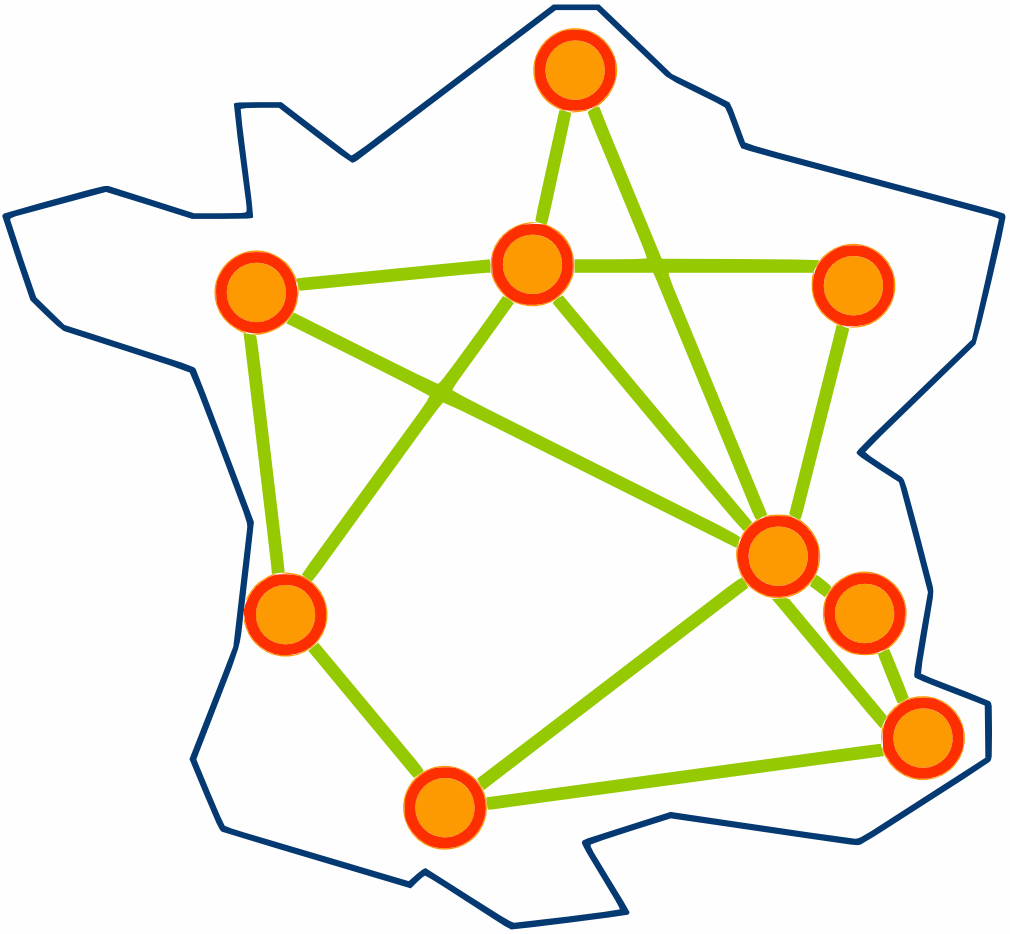
\includegraphics[width=0.4\linewidth]{images/Site_map.png}
				\caption{Les sites français du Grid'5000}
			\end{center}
		\end{figure}

		Chaque site possède un ou plusieurs clusters\footnote{TODO: def d'un cluster}. Par exemple, le site de Nancy possède deux clusters :
		
		\begin{description}
			\item[graphene :] 144 nœuds contenants :\\
			1 CPU Intel@2.53GHz\\
			4 cores/CPU\\
			16GB RAM\\
			278GB DISK
			\item[griffon :] 92 nœuds contenants :\\
			2 CPUs Intel@2.5GHz\\
			4 cores/CPU\\
			16GB RAM\\
			278GB DISK
		\end{description}


	\chapter{NFS}
		\section{Présentation}
		% FS distribué le plus simple ? (à mettre en place, dans ses possibilités) ?

		NFS (Network File System, système de fichiers en réseau en français) est un système de fichiers développé par Sun Microsystem,
		permettant de partager des données par le réseau. NFS est aujourd’hui la méthode standard de partage de disques entre machines Unix. 
		C’est une solution simple et pratique, quoique peu sécurisée.\\
		
		\section{Aspect technique}
		
		NFS utilise généralement le protocole non connecté UDP (en opposition à TCP qui est un pro-
    tocole connecté). Toutefois, certains clients et serveurs NFS (depuis la version 3) peuvent aussi
    utiliser TCP, ce qui permet, entre autre, de fiabiliser les échanges.\\

    On retrouve pour NFS différentes versions :\\
    NFSv1 et v2 définies dans la RFC 1094 prévues pour fonctionner sur UDP.\\
    NFSv3 définie dans la RFC 1813 prenant en charge le TCP.\\
    NFSv4 définie dans la RFC 3010 puis réviser dans la RFC 3530. L'ensemble du protocole est repensé, et les codes sont réécrits.
    Cette version intègre une meilleur gestion de la sécurité, de la montée en charge, et un systèmes de maintenances simplifiés.
    NFSv4 supporte les protocoles de transports TCP (par défaut) et RDMA, ce qui augmente la fiabilité. Nous utiliserons donc cette version
    NFS dans l'ensemble de nos test.\\
    
    \section{Mise en place}
    
    Dans cette configuration nous partageons un répertoire /tmp sur un serveur à plusieurs clients. Utilisant une image de Debian Squeeze,
    les paquets nfs-common et nfs-kernel-server sont directement disponible dans les dépôts. Il faut ensuite ajouter la ligne suivante dans
    le fichier /etc/exports :
    \begin{lstlisting}
	    /tmp *.nancy.grid5000.fr(rw,fsid=0,insecure,subtree_check)
	  \end{lstlisting}
	  Dans cette ligne le répertoire est partagé pour le domaine nancy.grid5000.fr. Cette manipulation n'est pas dutout sécurisé ! Puisque toutes
	  les machines déployées sur la plateforme de Nancy peuvent accéder au répertoire.\\
	  \textbf{rw }: autorise l'accès en lecture et écriture;\\
	  \textbf{fsid=0} : cette option est propre à NFSv4. Elle indique le point de partage racine. Ce qui permet de monter des partages en fonction d'une  
	  racine virtuelle.\\
	  \textbf{insecure} : l'option insecure permet l'accès aux clients dont l'implémentation NFS n'utilisent pas un port réservé.\\
	  \textbf{subtree\_check} : permet de limiter l'accès exclusivement au répertoire partager.\\
	  
	  Après la modification de ce fichier, il suffit de redémarrer le service, puis de monter les clients sur le répertoire partager à l'aide de la 
	  commande suivante :\\
	  \begin{lstlisting}
	    mount serveur:/ -t nfs4 /tmp/partage
	  \end{lstlisting}
	  Afin d'utiliser la version 4 de NFS, il est nécessaire de le spécifier dans le type lors du montage.\\
	\chapter{GlusterFs}
		\section{Présentation}
		% x serveurs, un maitre, mais ayant besoin des mêmes paquets que les autres
		% besoin d'un paquet pour les clients

	\chapter{MooseFS}
		% données temporaires, penser à citer les sources si passages copiés collés
		% il est apparemment aussi possible de mettre en place MooseFS sur un seul serveur
		\section{Présentation}

			\subsection{Présentation générale}
				% deux partie présentation ? Présentation générale, Présentation technique ?
		
				%MooseFS (Moose File System), un système de fichiers distribué. % enlever cette phrase ?
				
				MooseFS (Moose File System) est un système de fichiers répartis à tolérance de panne, développé par Gemius SA
				Le code préalablement propriétaire a été libéré et mis à disposition publiquement le 5 mai 2008.
				Il permet de déployer assez facilement un espace de stockage réseau, répartit sur plusieurs serveurs.
				
				Cette répartition permet de gérer la disponibilité des données,
				lors des montées en charge ou lors d’incident technique sur un serveur.
				L'atout principal de MooseFS, au delà du fait qu'il s’agisse d’un logiciel libre, est sa simplicité de mise en œuvre.
				% plus simple à mettre en place que les autres ?
				
				En effet le tutoriel de prise en main, disponible sur le site du projet,
				explique de manière clair comment mettre en place une architecture distribuées en quelques heures.
				Concernant les utilisations, elles sont multiples et surtout, après la phase de configuration,
				l'évolution du système est très simple. L'ajout de serveurs, d’espace disque peuvent être gérés très facilement.

			\subsection{Aspect technique}
				
				Les montage du système de fichiers par les clients se fait à l'aide de FUSE. % deux trois mots sur FUSE ?

				MooseFS est constitué de trois types de serveurs :

				\begin{enumerate}
					\item Un serveur de métadonnées (MDS)

					Ce serveur gère la répartition des différents fichiers
					\item Un serveur métajournal (Metalogger server)

					Ce serveur récupère régulièrement les métadonnées du MDS et les stocke en tant que sauvegarde.
					\item Des serveurs Chunk (CSS) % pourquoi CSS ?

					Ce sont ces serveurs qui stockent les données des utilisateurs.
				\end{enumerate}
				
				Le point le plus important étant de bien dimensionner le serveur Master (qui stocke les méta-données)
				afin de ne pas être limité par le suite.\\

				MooseFS permet de partager des données sur plusieurs machines de manière rapide, fiable et sécurisée.

		\section{Mise en place}
			\subsection{Environnement logiciel}

				Le système utilisé est une Debian Squeeze. MooseFs ne faisant pas partie des dépôts de la distribution,
				nous avons compilé le paquet à partir des sources dans leurs dernières version (1.6.20).
				% Deban Squeeze + MooseFS version x compilé depuis les sources (pas présent dans les dépôts),
				% avec options différentes suivant les serveurs, clients (cf tuto site officiel)

		

% insertion d'une image :
%\begin{figure}[p]
%	\includegraphics[width=12cm,height=120mm]{mastersrv.png}
%	\caption{MooseFs Read Process}
%	\label{identifiant test}
%\end{figure} 

	\chapter{Ceph}
		\section{Présentation}

	\chapter{Comparaison}
	% comparaison des performances
	% aspects générales, site officiel (doc, tuto), avis personnels
		\section{Test de performances}
			Afin de ne pas avoir de différence de matériel lors nos test, ceux-ci ont tous été réalisés sur un même cluster du Grid'5000 : Graphene.\\

			Ce cluster est composé de 144 noeuds, avec pour caractéristique :
			\begin{itemize}
				\item 1 CPU Intel de quatre cœurs cadencé à 2.53 GHz
				\item 16 Go de RAM
				\item 278 Go d'espace disque\\
			\end{itemize}

			Nous avons réalisé un benchmark mesurant les performances (débit) de quatre type d'opérations sur le système de fichier distribué :
			\begin{description}
				\item[Écriture de petits fichiers :] écriture des sources du noyau linux (décompressé).
				\item[Écriture de gros fichiers :] écriture d'un fichier de 3 Go\footnote{Fichier créé avec la commande : dd if=/dev/zero of=/lieu/voulu bs=1G count=3}.
				\item[Lecture de petits fichiers: ] lecture des fichiers du noyau linux.
				Pour cela, nous avons compressé le dossier contenant le noyau (impliquant la lecture des fichiers),
				en redirigeant la sortie vers /dev/nul (afin que les performances du disque ne rentrent pas en jeux).
				\item[Lecture de gros fichiers :] lecture du fichier de 3 Go. Opération réalisé en faisant un "cat" du fichier,
				et en redirigeant la sortie vers /dev/nul afin de ne pas "polluer" le terminal.
			\end{description}


	\chapter{Conclusion}
	% sur les FS
	% sur nos objectifs de départ
	% apport du projet tuteuré pour nous, bonne expérience avant départ en stage, ...

	\appendix
		\chapter{Répartition des taches}
			\section{Florent Lévigne}
				\begin{itemize}
					\item Étude sur la mise en place de GlusterFS
					\item Réalisation d'un script de déploiement de GlusterFS
					\item Étude sur la mise en place de MooseFS
					\item Réalisation d'un script de déploiement de MooseFS
					\item Réalisation d'un script de benchmark pour système de fichiers distribué
				\end{itemize}
			\section{Jean-François Garcia}
				\begin{itemize}
					\item Étude sur la mise en place de GlusterFS
					\item Étude sur la mise en place de NFS
					\item Réalisation d'un script de déploiement de NFS
					\item Étude sur la mise en place de CephFS
					\item Réalisation d'un script de déploiement de CephFS
				\end{itemize}

		\chapter{Scripts}
			\section{GlusterFs}
				Fichier deploimentGluster.rb :
				\lstinputlisting[language=Ruby]{../glusterFs/deploiementGluster.rb}
				% autre fichier (améliorer le script)
			\section{MooseFs}
			\section{Ceph}
			  Fichier deploimentCeph.rb :
				\lstinputlisting[language=Ruby]{../cephFS/deploiementCeph.rb}
			\section{NFS}
			  Fichier deploimentNFS.rb :
				\lstinputlisting[language=Ruby]{../NFS/deploiementNFS.rb}
			\section{Benchmark}
				Fichier benchmark.rb :
				\lstinputlisting[language=Ruby]{../benchmark/benchmark.rb}

				Fichier writingSmallFiles.sh :
				\lstinputlisting[language=Bash]{../benchmark/writingSmallFiles.sh}

				Fichier writingBigFiles.sh :
				\lstinputlisting[language=Bash]{../benchmark/writingBigFiles.sh}

				Fichier readingSmallFiles.sh :
				\lstinputlisting[language=Bash]{../benchmark/readingSmallFiles.sh}

				Fichier readingBigFile.sh :
				\lstinputlisting[language=Bash]{../benchmark/readingBigFile.sh}
\end{document}

